\documentclass[a4paper]{article}

\usepackage[pdftex]{graphicx}
\usepackage[margin=3cm]{geometry}
\usepackage{verbatim,moreverb,amssymb,amsmath}


\newcounter{question}
\newcommand{\question}[1]{\refstepcounter{question}\section*{Question~\thequestion~~~\small\emph{(#1)}}}
\renewcommand*\thequestion{\arabic{question}}


\begin{document}

\pagestyle{empty}
\thispagestyle{empty}



\noindent
\begin{minipage}{\columnwidth}
  \centering
  \Large
  DA4002 (HT11) Halmstad University\\
  Introduction to Algorithms, Data Structures, and Problem Solving\\[3\baselineskip]
  \Huge
  Written Exam\\
  \Large
  Thursday, August 22, 2013\\[2\baselineskip]
  Examiner: Roland Philippsen
\end{minipage}

\vfill

\noindent
\begin{center}
\fbox{
  \begin{minipage}{0.8\columnwidth}
    \textbf{Student Name:}\\[3\baselineskip]
  \end{minipage}
}
\end{center}

\vfill



\section*{Rules}

Aside from the obvious rules of conduct exams (e.g.\ no chatting):

\begin{itemize}
\item
  \textbf{No computing devices} (laptops, phones, calculators, \emph{etc}).
\item
  \textbf{No books or printouts} except for non-electronic dictionaries.
\item
  \textbf{Allowed hand-written notes}: two sheets of A4 paper (front and back).
\end{itemize}



\section*{General Guidelines}

\begin{itemize}
\item
  \textbf{Read carefully} and pace yourself.
  You can solve the problems in any order you want, but later problems may be easier to solve after you have answered the preceding questions.
\item
  \textbf{Write clearly} and draw clear diagrams.
  If you need to correct a mistake, then cleanly cross out the wrong answer and clearly indicate where the correction can be found.
\item
  \textbf{Indicate the question number} for each of your answers.
  If a question has sub-questions, indicate the sub-question number after the main question number, separated by a dot.
  For example, question 3 has 4 sub-questions, and their answers should be numbered 3.1, 3.2, 3.3, and 3.4.
\end{itemize}



\pagebreak
\pagestyle{plain}
\thispagestyle{plain}
\setcounter{page}{1}



\question{6 points}

\begin{enumerate}
\item
  Draw an example diagram for each of the following data structure types:
  \begin{enumerate}
  \item
    simply linked list
  \item
    doubly linked list
  \item
    binary tree
  \item
    directed acyclic graph
  \end{enumerate}
\item
  For each of the two following diagrams, explain why it is \textbf{not} a valid example of any of the above data structure types.
\end{enumerate}

\begin{center}
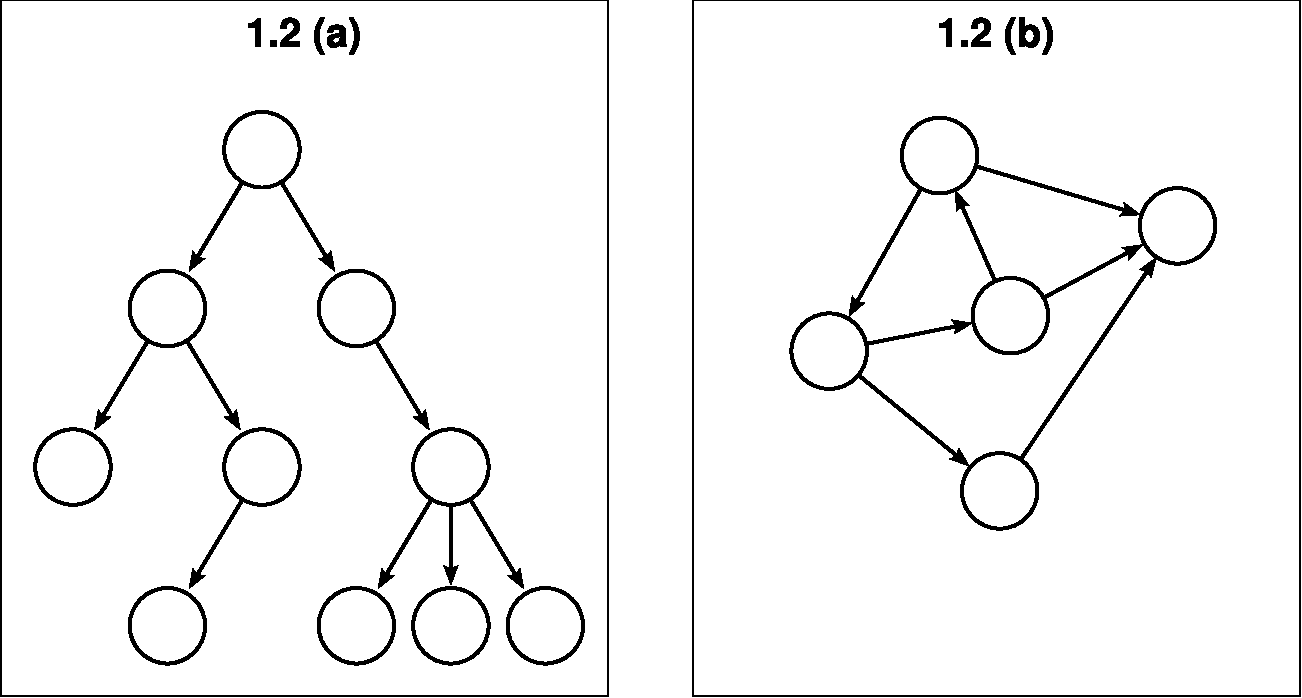
\includegraphics[width=0.6\columnwidth]{q1.pdf}
\end{center}


\clearpage


\question{6 points}

The following C code contains a tree data structure type declaration and three traversal functions.
Note that the \texttt{Fifo} data structure and the various \texttt{fifo\_} functions provide a first-in first-out queue whose implementation is not shown.

\begin{enumerate}
\item
  For each of the functions, write down whether it does pre-order, post-order, in-order, or level-order traversal.
\item
  Given the example tree in the diagram below, write down for each function the sequence of characters that it prints out.
  Note that the non-labeled horizontal arrows are the \texttt{sbl} pointers, the non-labeled downward-pointing arrows are \texttt{cld} pointers, and \texttt{\textsc{null}}-pointers are not shown.
\end{enumerate}

\noindent
\fbox{\begin{minipage}[b]{0.65\columnwidth}
  \small
  \verbatimtabinput{q2-pseudocode.c}
\end{minipage}}%
\hfill%
\fbox{\begin{minipage}[b]{0.3\columnwidth}
    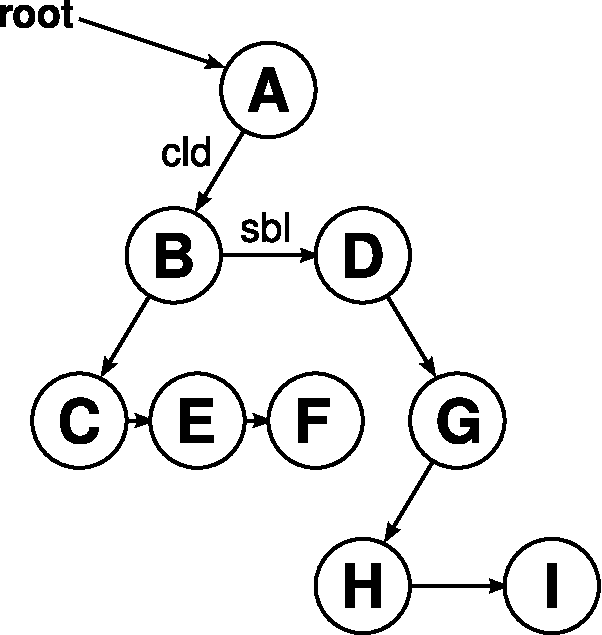
\includegraphics[width=\columnwidth]{q2.pdf}
\end{minipage}}


\clearpage


\question{4 points}

\emph{Hint: there is a lookup table for powers of 2 at the bottom of the page.}

\begin{enumerate}

\item
  What is the runtime complexity of the following \texttt{algo\_a}?
  Note that the \texttt{Item} structure is a simply linked list element containing an integer \texttt{num} and a pointer to the next element.
  There are $N$ elements in the list, and the last element has a \texttt{next} pointer which is \texttt{\textsc{null}}.
  
  \fbox{\begin{minipage}{0.65\columnwidth}\verbatimtabinput{q3-snip1.c}\end{minipage}}

\item
  What is the runtime complexity of the following \texttt{algo\_b}?
  Like before, it also receives a simply linked list with $N$ elements.
  
  \fbox{\begin{minipage}{0.65\columnwidth}\verbatimtabinput{q3-snip2.c}\end{minipage}}

\item
  Algorithm C (code not shown) is known to have $N\log N$ runtime complexity.
  It has been measured to require 10 seconds on a problem of size 1024.
  How long can it be expected to run on a problem of size 4096?
  
\item
  Algorithm D (code not shown) is known to have exponential runtime complexity.
  It requires 1 second to solve a problem of size 2048.
  How big of a problem can be solved if we are willing to wait 4096 seconds?
\end{enumerate}

\vfill

\begin{tabular}{|l|r|r|r|r|r|r|r|r|r|r|r|r|r|r|r|}
  \hline
  $x=$   & 0 & 1 & 2 & 3 & 4 & 5 & 6 & 7 & 8 & 9 & 10 & 11 & 12 & 13 & 14 \\
  \hline
  $2^x=$ & 1 & 2 & 4 & 8 & 16 & 32 & 64 & 128 & 256 & 512 & 1024 & 2048 & 4096 & 8192 & 16384 \\
  \hline
\end{tabular}


\clearpage


\question{5 points}

In the following program, \texttt{print} is a function to print a number sequence defined recursively.
The \texttt{calc} function is a straightforward but inefficient implementation to compute the members of that sequence.

\begin{enumerate}
\item
  How many times will \texttt{calc(3)} get called as a result of calling \texttt{print(6)}?
\item
  Use \emph{memoization} to implement a more efficient version of \texttt{calc}.
  You can give your answer in pseudo-code or as a textual explanation, there is no need to create correct C code.
\item
  Use \emph{dynamic programming} to implement an iterative version of \texttt{calc}.
  Again, you can give your answer in pseudo-code or as a textual explanation.
\end{enumerate}

\noindent
\fbox{\begin{minipage}{0.65\columnwidth}\verbatimtabinput{q4.c}\end{minipage}}


\clearpage


\question{4 points}

\begin{enumerate}
\item
  The \texttt{find} function shown below contains an error.
  It is supposed to implement binary search on an array of integers that is in ascending order.
  The idea is to return the index where the given \texttt{num} is stored, or -1 in case that number is not in the array \texttt{arr} of length \texttt{len}.
  But, for example on the array \{1, 23, 25, 66, 102\} it fails to find the number 66.
  What is the problem, and how can it be fixed?
  
  \fbox{\begin{minipage}{0.65\columnwidth}\verbatimtabinput{q5a.c}\end{minipage}}
  
\item
  There also is a bug in the \texttt{sort} function shown below.
  It is supposed to implement insertion sort on an array of integers.
  But, for example on the array \{ 6, 0, 7, 3, 8, 5, 1, 4, 9, 2 \} it produces the incorrect output \{ 6, 6, 7, 7, 8, 8, 8, 8, 9, 9 \}.
  What is wrong, and how can it be fixed?
  
  \fbox{\begin{minipage}{0.65\columnwidth}\verbatimtabinput{q5b.c}\end{minipage}}
  
\end{enumerate}


\end{document}
